% =============================================================================
% In a Different Voice: Gender Composition and Scientific Writing in Economics
% Conference presentation — ~20 minutes — 12 frames
% Cassar, Coffelt, Datuashvili, Khubulashvili
% =============================================================================

\documentclass[aspectratio=169,11pt]{beamer}

\usepackage[utf8]{inputenc}
\usepackage[T1]{fontenc}
\usepackage{lmodern}
\usepackage{microtype}
\usepackage{amsmath,amssymb}
\usepackage{booktabs}
\usepackage{graphicx}
\usepackage{tikz}
\usepackage{xcolor}
\usepackage{ragged2e}
\usepackage{colortbl}
\usepackage{array}
\usepackage{hyperref}
\usepackage{adjustbox}
\usepackage[normalem]{ulem}

\pgfkeys{/pgf/.cd}

% --- Color Palette: Warm Professional ---
\definecolor{DeepNavy}{HTML}{2E4057}
\definecolor{Teal}{HTML}{048A81}
\definecolor{WarmOrange}{HTML}{E85D04}
\definecolor{SoftPurple}{HTML}{9D4EDD}
\definecolor{WarmGray}{HTML}{6C757D}
\definecolor{LightGray}{HTML}{E9ECEF}
\definecolor{DeepRed}{HTML}{D62828}
\definecolor{Gold}{HTML}{D4A03A}
\definecolor{SoftWhite}{HTML}{FAFAFA}

% Beamer colors
\setbeamercolor{normal text}{fg=DeepNavy, bg=SoftWhite}
\setbeamercolor{structure}{fg=DeepNavy}
\setbeamercolor{alerted text}{fg=DeepRed}
\setbeamercolor{frametitle}{fg=DeepNavy, bg=SoftWhite}
\setbeamercolor{title}{fg=DeepNavy}
\setbeamercolor{subtitle}{fg=WarmGray}
\setbeamercolor{block title}{bg=DeepNavy, fg=SoftWhite}
\setbeamercolor{block body}{bg=LightGray, fg=DeepNavy}

% Fonts
\usefonttheme{professionalfonts}
\setbeamerfont{title}{size=\huge, series=\bfseries}
\setbeamerfont{frametitle}{size=\Large, series=\bfseries}

% Strip chrome
\setbeamertemplate{navigation symbols}{}
\setbeamertemplate{headline}{}

% Footline
\setbeamertemplate{footline}{%
    \hfill
    \begin{beamercolorbox}[wd=3cm,ht=2.5ex,dp=1ex,right,rightskip=0.6cm]{normal text}
        \color{WarmGray}\scriptsize\insertframenumber
    \end{beamercolorbox}
    \vspace{0.3cm}
}

\graphicspath{{figures/}}

% =============================================================================
\begin{document}
% =============================================================================

% ---------------------------------------------------------------------------
% 1. Title
% ---------------------------------------------------------------------------
\begin{frame}[plain]
    \vfill
    \centering
    {\huge\bfseries\color{DeepNavy} In a Different Voice}\\[0.4cm]
    {\large\color{WarmGray} Gender Composition and Scientific Writing in Economics}\\[0.8cm]
    \textcolor{LightGray}{\rule{0.5\textwidth}{0.4pt}}\\[0.5cm]
    {\normalsize\color{DeepNavy}
        Alessandra Cassar \quad Austin Coffelt \quad
        Sopiko Datuashvili \quad Robizon Khubulashvili}\\[0.2cm]
    {\small\color{WarmGray} University of San Francisco \quad$\cdot$\quad April 2026}
    \vfill
\end{frame}

% ---------------------------------------------------------------------------
% 2. Motivation & Research Question
% ---------------------------------------------------------------------------
\begin{frame}{Scientific writing is not a neutral container for ideas}
    \vfill
    \RaggedRight
    {\normalsize\color{WarmGray}\textit{How research is framed shapes evaluation --- dominant standards may systematically overlook a ``different voice'' (Gilligan 1993)}}
    \vspace{0.25cm}

    {\normalsize
    \begin{itemize}\setlength\itemsep{0.18cm}
        \item Does gender composition predict systematic differences in how economists write?
        \item Builds on Hengel (2022) \textit{Publishing While Female}: female-authored papers more readable; writing gap widens during peer review
        \item Extends to \textbf{15 additional} tonal dimensions --- assertiveness, hedging, directness, novelty claims, and more
    \end{itemize}
    }
    \vspace{0.22cm}
    {\small\bfseries\color{Teal} Preview of findings}\\[0.1cm]
    {\normalsize
    \begin{itemize}\setlength\itemsep{0.15cm}
        \item Clarity gap: female-majority teams score higher on readability, directness, and evidentiary support; lower on jargon
        \item Tonal dimensions --- assertiveness, hedging, emotional valence --- no systematic difference
    \end{itemize}
    }
    \vfill
\end{frame}

% ---------------------------------------------------------------------------
% 3. Related Literature
% ---------------------------------------------------------------------------
\begin{frame}{This paper contributes to three literatures}
    \vfill
    \RaggedRight
    {\normalsize
    \begin{itemize}\setlength\itemsep{0.3cm}
        \item \textbf{Gender, voice, \& communication} --- Gilligan (1993): dominant evaluative standards may systematically overlook a ``different voice''
        \item \textbf{Gender and economics outcomes} --- Card et al.\ (2020): referees treat submissions differently by gender; Sarsons (2017): collaborative work differentially credited
        \item \textbf{Readability and peer review} --- Hengel (2022) \textit{Publishing While Female}: female-authored papers more readable; writing gap widens during review
        \item \textbf{Our contribution} --- extend Hengel with 15 additional tonal dimensions; sharpen the ``different voice'' debate by identifying \textit{which} dimensions move with team composition
    \end{itemize}
    }
    \vfill
\end{frame}

% ---------------------------------------------------------------------------
% 4. Data
% ---------------------------------------------------------------------------
\begin{frame}{9,117 abstracts from four top economics journals, 1950--2015}
    \vfill
    \RaggedRight
    {\normalsize
    \begin{itemize}\setlength\itemsep{0.28cm}
        \item Source: Hengel (2022) replication dataset --- \textit{AER}, \textit{ECA}, \textit{JPE}, \textit{QJE}, 1950--2015; analysis on abstracts only
        \item \textbf{Article-level controls}: JEL codes, submission \& acceptance dates, citation count, pre-computed readability scores, blind-review indicator
        \item \textbf{Author-level controls}: gender, native language, institution, seniority, prominence (most-published co-author)
        \item Sample: 7,939 all-male articles, 319 all-female; $<\!10\%$ female authors overall
        \item Six authorship measures: female ratio, majority female, any female, 100\% female, solo female, senior female
    \end{itemize}
    }
    \vfill
\end{frame}

% ---------------------------------------------------------------------------
% 5. Rubric
% ---------------------------------------------------------------------------
\begin{frame}{16-item LLM rubric: surface-level linguistic features only}
    \vspace{0.1cm}
    {\normalsize\color{WarmGray} Each criterion scored 1--10. No author intent or personality inferred.}
    \vspace{0.3cm}

    \begin{columns}[T, onlytextwidth]

        \begin{column}{0.48\textwidth}
            \RaggedRight
            {\normalsize
            \textbf{\color{Teal} G1} Creativity \& Hedging\\[0.05cm]
            {\small\color{WarmGray} Modal Verb, Hedging, Qualifier Density, Ack.\ of Limitations, Caution}
            \vspace{0.25cm}

            \textbf{\color{WarmOrange} G2} Assertiveness \& Voice\\[0.05cm]
            {\small\color{WarmGray} Assertiveness, Active/Passive Voice}
            \vspace{0.25cm}

            \textbf{\color{SoftPurple} G3} Structural Directness\\[0.05cm]
            {\small\color{WarmGray} Sentence Directness, Imperative-Form Occurrence}
            }
        \end{column}

        \begin{column}{0.04\textwidth}\end{column}

        \begin{column}{0.48\textwidth}
            \RaggedRight
            {\normalsize
            \textbf{\color{Gold} G4} Authorial Stance \& Novelty\\[0.05cm]
            {\small\color{WarmGray} Pronoun Commitment, Novelty Claims, Jargon Density, Emotional Valence}
            \vspace{0.25cm}

            \textbf{\color{DeepRed} G5} Support \& Impact\\[0.05cm]
            {\small\color{WarmGray} Evidence \& Citation Usage, Practical Orientation}
            \vspace{0.25cm}

            \textbf{\color{WarmGray} Standalone} Readability
            }
        \end{column}

    \end{columns}
    \vspace{0.3cm}
    {\small\color{WarmGray} $^{\dagger}$Jargon/Technicality Density is scale-flipped ($11-$raw) so that high score $=$ less jargon.}
\end{frame}

% ---------------------------------------------------------------------------
% 6. LLM Evaluations
% ---------------------------------------------------------------------------
\begin{frame}{GPT-5 with chain-of-thought reasoning scored all 9,117 abstracts}
    \vfill
    {\normalsize
    \begin{itemize}\setlength\itemsep{0.3cm}
        \item \textbf{Model:} GPT-5 — extended reasoning before answering improves accuracy on complex tasks (Shojaee et al.\ 2025)
        \item \textbf{Pipeline:} abstract $\rightarrow$ rubric $\rightarrow$ model $\rightarrow$ structured 16-score output
        \item \textbf{Prompt engineering:} step-by-step reasoning induced per criterion; shorter inputs increase accuracy (Modarressi et al.\ 2025)
        \item \textbf{Validation:} human-in-the-loop on small subset --- audited outputs and iteratively improved prompt; then benchmarked against Hengel (2022) readability scores
        \item {\color{WarmGray}\textit{Caveat:} some randomness in LLM outputs; reported SEs may understate true uncertainty}
    \end{itemize}
    }
    \vfill
\end{frame}

% ---------------------------------------------------------------------------
% 7. Empirical Strategy
% ---------------------------------------------------------------------------
\begin{frame}{Three-step analysis: validate $\rightarrow$ mean differences $\rightarrow$ controlled regressions}
    \vfill
    \begin{center}
        {\normalsize
        \textbf{(1)} Benchmark LLM readability against Hengel (2022) measures\quad
        \textbf{(2)} Unconditional mean differences across all 16 criteria\quad
        \textbf{(3)} Controlled regressions
        }
    \end{center}
    \vspace{0.4cm}
    \begin{center}
        {\large
        $R_j = \beta_0 + \beta_1 \cdot \textit{FemaleRatio}_j
             + \gamma X_j + \delta Y_j + \varepsilon_j$}
    \end{center}
    \vspace{0.4cm}
    \begin{columns}[T, onlytextwidth]
        \begin{column}{0.48\textwidth}
            \RaggedRight
            {\normalsize
            $X_j$: journal$\times$year FE, editor controls, blind-review indicator, JEL codes, theory/empirical flag}
        \end{column}
        \begin{column}{0.04\textwidth}\end{column}
        \begin{column}{0.48\textwidth}
            \RaggedRight
            {\normalsize
            $Y_j$: institution FE, author prominence (max $T$ FE), author seniority (max $t$ FE), native-speaker indicator}
        \end{column}
    \end{columns}
    \vspace{0.4cm}
    \begin{center}
        {\small\color{WarmGray}
        Nine specifications. SEs clustered on editor. Alternative authorship measures: majority-female binary, any-female binary, 100\% female, solo, senior female.}
    \end{center}
    \vfill
\end{frame}

% ---------------------------------------------------------------------------
% 8. Results 5.1 — Benchmarking
% ---------------------------------------------------------------------------
\begin{frame}{LLM readability replicates Hengel's established pattern across all nine specifications}
    \vfill
    \begin{center}
    {\small
    \begin{tabular}{lcc}
        \toprule
        Readability measure & (4) & (5) \\
        \midrule
        Flesch Reading Ease             & $1.26^{**}$  & $1.49^{***}$ \\
        Flesch-Kincaid Grade Level      & $0.24^{*}$   & $0.26^{*}$   \\
        Gunning Fog Index               & $0.40^{**}$  & $0.42^{***}$ \\
        SMOG Index                      & $0.27^{**}$  & $0.29^{**}$  \\
        Dale-Chall Score                & $0.08$       & $0.09$       \\
        \midrule
        \textbf{LLM Readability}        & $\mathbf{0.40^{***}}$ & $\mathbf{0.32^{***}}$ \\
        \midrule
        $N$                             & 9,117        & 9,117        \\
        \bottomrule
    \end{tabular}
    }
    \end{center}
    \vspace{0.3cm}
    \begin{center}
        {\small\color{WarmGray}
        OLS coefficients on female ratio. SEs clustered on editor.
        Col.~(4): journal$\times$year, $N_j$, institution, editor, blind-review.
        Col.~(5) adds quality controls, native speaker, JEL, theory/empirical.}
    \end{center}
    \vfill
\end{frame}

% ---------------------------------------------------------------------------
% 9. Results 5.2 — Mean differences
% ---------------------------------------------------------------------------
\begin{frame}{Female-majority teams score higher on clarity; tonal differences are negligible}
    \vspace{-0.2cm}
    \begin{center}
        \adjustbox{max width=\textwidth, max height=0.63\textheight}{%
            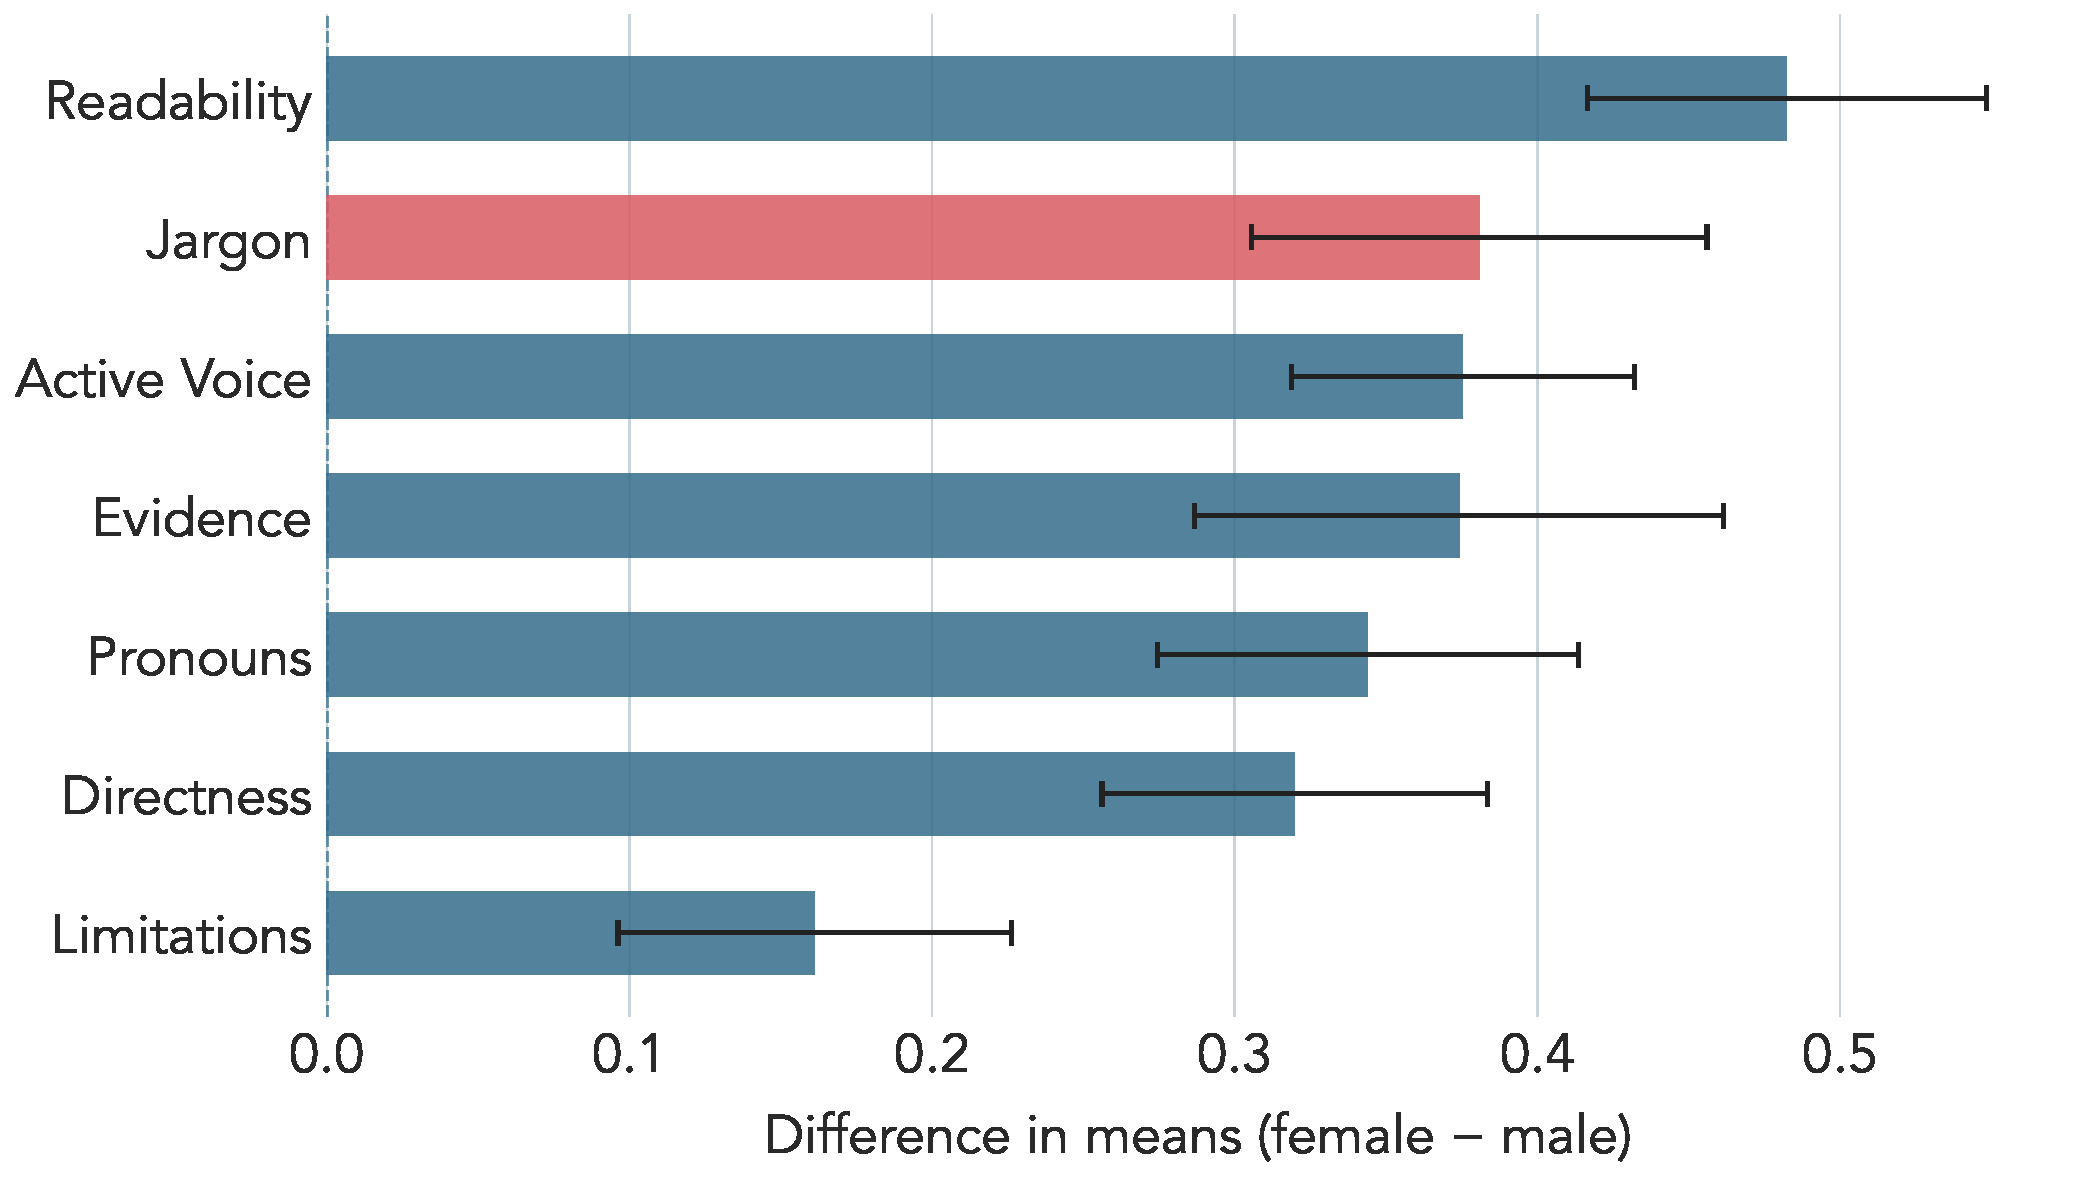
\includegraphics{diff_means_plot_slides.pdf}%
        }
    \end{center}
    \begin{center}
        {\small\color{WarmGray} Null: assertiveness, hedging, emotional valence --- no difference between male- and female-majority teams.}
    \end{center}
\end{frame}

% ---------------------------------------------------------------------------
% 10. Results 5.3 — Controlled regressions
% ---------------------------------------------------------------------------
\begin{frame}{Controlled regressions confirm the clarity differential; tonal dimensions remain null}
    \vfill
    \begin{center}
    {\small
    \begin{tabular}{lcc}
        \toprule
        Criterion & (4) & (5) \\
        \midrule
        Jargon/Technicality Density$^{\dagger}$ & $0.55^{***}$ & $0.48^{***}$ \\
        Sentence Length \& Directness           & $0.31^{***}$ & $0.25^{**}$  \\
        Evidence \& Citation Usage              & $0.46^{***}$ & $0.36^{***}$ \\
        Pronoun Commitment                       & $0.39^{**}$  & $0.32$       \\
        Acknowledgement of Limitations          & $0.24^{**}$  & $0.15$       \\
        Active/Passive Voice                     & $0.16$       & $0.15$       \\
        \midrule
        $N$                                      & 9,117        & 9,117        \\
        \bottomrule
    \end{tabular}
    }
    \end{center}
    \vspace{0.2cm}
    \begin{center}
        {\small\color{WarmGray}
        OLS coefficients on female ratio. SEs clustered on editor.
        Col.~(4): journal$\times$year, $N_j$, institution, editor, blind-review.
        Col.~(5) adds quality controls, native speaker.
        $^{\dagger}$Scale-flipped (11$-$raw); positive $=$ less jargon.}
    \end{center}
    \vfill
\end{frame}

% ---------------------------------------------------------------------------
% 11. Robustness
% ---------------------------------------------------------------------------
\begin{frame}{Clarity differential is robust across six authorship measures}
    \vfill
    \begin{center}
    {\small
    \begin{tabular}{lcccccc}
        \toprule
        & \multicolumn{6}{c}{Authorship measure} \\
        \cmidrule(lr){2-7}
        Criterion
            & \shortstack[c]{Female\\ratio}
            & \shortstack[c]{$\geq$50\%\\female}
            & \shortstack[c]{$\geq$1\\female}
            & \shortstack[c]{100\%\\female}
            & \shortstack[c]{Solo\\female}
            & \shortstack[c]{Senior\\female} \\
        \midrule
        \textbf{LLM Readability}          & $0.32^{***}$ & $0.22^{***}$ & $0.18^{***}$ & $0.31^{***}$ & $0.26^{**}$  & $0.33^{***}$ \\
        Jargon/Technicality$^{\dagger}$   & $0.48^{***}$ & $0.31^{***}$ & $0.28^{***}$ & $0.51^{***}$ & $0.45^{***}$ & $0.57^{***}$ \\
        Sentence Directness               & $0.25^{**}$  & $0.20^{**}$  & $0.17^{***}$ & $0.21^{*}$   & $0.16$       & $0.21^{**}$  \\
        \midrule
        Assertiveness                     & $-0.05$      & $-0.00$      & $-0.02$      & $-0.13$      & $-0.16$      & $-0.14$      \\
        Emotional Valence                 & $-0.03$      & $-0.02$      & $-0.01$      & $-0.04^{*}$  & $-0.04^{**}$ & $-0.03^{*}$  \\
        \midrule
        $N$                               & \multicolumn{6}{c}{9,117} \\
        \bottomrule
    \end{tabular}
    }
    \end{center}
    \vspace{0.2cm}
    \begin{center}
        {\small\color{WarmGray}
        OLS col~(5) coefficients on authorship measure. SEs clustered on editor.
        $^{\dagger}$Scale-flipped (11$-$raw); positive $=$ less jargon.}
    \end{center}
    \vfill
\end{frame}

% ---------------------------------------------------------------------------
% 12. Conclusion
% ---------------------------------------------------------------------------
{\setbeamercolor{background canvas}{bg=DeepNavy}
\begin{frame}[plain]
    \vfill
    \begin{center}
        {\LARGE\bfseries\color{SoftWhite}
        Female-majority teams in economics\\[0.3cm]
        write more \textcolor{Gold}{clearly}.}\\[0.6cm]
        \textcolor{WarmGray}{\rule{0.45\textwidth}{0.4pt}}\\[0.5cm]
        {\large\color{LightGray}
        LLM readability validates against Hengel (2022). In mean differences and controlled regressions,
        female-majority teams score higher on readability, directness, active voice, and evidentiary support,
        and lower on jargon --- not more hesitant or emotional.
        Robust across control levels and authorship specifications;
        LLM measurement error not yet fully quantified.}
    \end{center}
    \vfill
\end{frame}
}

% ---------------------------------------------------------------------------
% 13. Thank you / Questions
% ---------------------------------------------------------------------------
{\setbeamercolor{background canvas}{bg=DeepNavy}
\begin{frame}[plain]
    \vfill
    \begin{center}
        {\Huge\bfseries\color{SoftWhite} Thank you.}\\[0.8cm]
        \textcolor{WarmGray}{\rule{0.35\textwidth}{0.4pt}}\\[0.8cm]
        {\LARGE\color{Gold} Questions?}
    \end{center}
    \vfill
\end{frame}
}

% ===========================================================================
% Appendix slides
% ===========================================================================
\appendix

\begin{frame}{Appendix: Summary statistics by gender composition}
    \RaggedRight
    \begin{center}
    {\small
    \begin{tabular}{lcccc}
        \toprule
        & All-Male & Mixed & All-Female & Full\\
        & ($N=7{,}951$) & ($N=853$) & ($N=313$) & ($N=9{,}117$)\\
        \midrule
        Readability    & 6.70 (1.38) & 7.42 (1.25) & 7.37 (1.30) & 6.79 (1.38)\\
        Directness     & 5.94 (2.08) & 6.71 (1.81) & 6.53 (1.86) & 6.03 (2.06)\\
        Jargon (raw)   & 7.00 (1.73) & 6.48 (1.86) & 6.07 (1.92) & 6.92 (1.76)\\
        Evidence       & 1.68 (1.34) & 2.31 (1.90) & 2.19 (1.73) & 1.75 (1.43)\\
        Novelty        & 2.27 (2.12) & 2.26 (2.20) & 1.90 (1.85) & 2.25 (2.12)\\
        Assertiveness  & 8.18 (1.55) & 8.43 (1.28) & 8.04 (1.55) & 8.20 (1.53)\\
        Hedging        & 8.35 (1.98) & 8.49 (1.73) & 8.07 (2.11) & 8.35 (1.96)\\
        Emotional val. & 1.12 (0.37) & 1.11 (0.35) & 1.10 (0.31) & 1.12 (0.37)\\
        \bottomrule
    \end{tabular}
    }
    \end{center}
    {\small\color{WarmGray} Means and SDs. Scored 1--10. Descriptive only; no significance stars.}
\end{frame}

% ---------------------------------------------------------------------------
% Backup A: col 4+5, G1+G2 tonal criteria not on slide 10
% ---------------------------------------------------------------------------
\begin{frame}{Appendix: Tonal criteria — controlled regressions (G1--G2)}
    \vfill
    \begin{center}
    {\small
    \begin{tabular}{lcc}
        \toprule
        Criterion & (4) & (5) \\
        \midrule
        Modal Verb Strength               & $-0.32^{*}$  & $-0.34^{*}$  \\
        Hedging Frequency \& Type         & $-0.20^{*}$  & $-0.17$      \\
        Qualifier Density                 & $0.00$       & $0.01$       \\
        Caution-Signaling Connectors      & $0.08$       & $0.08$       \\
        Assertiveness \& Voice            & $-0.06$      & $-0.05$      \\
        \midrule
        $N$                               & \multicolumn{2}{c}{9,117} \\
        \bottomrule
    \end{tabular}
    }
    \end{center}
    \vspace{0.2cm}
    \begin{center}
        {\small\color{WarmGray}
        OLS coefficients on female ratio. SEs clustered on editor.
        Col.~(4): journal$\times$year, $N_j$, institution, editor, blind-review.
        Col.~(5) adds quality controls, native speaker, JEL, theory/empirical.}
    \end{center}
    \vfill
\end{frame}

% ---------------------------------------------------------------------------
% Backup B: col 4+5, remaining criteria not on slide 10
% ---------------------------------------------------------------------------
\begin{frame}{Appendix: Remaining criteria — controlled regressions (G3--G5)}
    \vfill
    \begin{center}
    {\small
    \begin{tabular}{lcc}
        \toprule
        Criterion & (4) & (5) \\
        \midrule
        Imperative-Form Occurrence        & $-0.02^{***}$ & $-0.02^{***}$ \\
        Novelty-Claim Strength            & $-0.31^{***}$ & $-0.30^{***}$ \\
        Emotional Valence                 & $-0.03$       & $-0.03$       \\
        Practical/Impact Orientation      & $0.09$        & $0.05$        \\
        \midrule
        $N$                               & \multicolumn{2}{c}{9,117} \\
        \bottomrule
    \end{tabular}
    }
    \end{center}
    \vspace{0.2cm}
    \begin{center}
        {\small\color{WarmGray}
        OLS coefficients on female ratio. SEs clustered on editor.
        Col.~(4): journal$\times$year, $N_j$, institution, editor, blind-review.
        Col.~(5) adds quality controls, native speaker, JEL, theory/empirical.}
    \end{center}
    \vfill
\end{frame}

% ---------------------------------------------------------------------------
% Backup C: col 5 × 6 specs, G1+G2 criteria not on slide 11
% ---------------------------------------------------------------------------
\begin{frame}{Appendix: Tonal criteria — robustness across authorship specifications (G1--G2)}
    \vfill
    \begin{center}
    {\small
    \begin{tabular}{lcccccc}
        \toprule
        & \multicolumn{6}{c}{Authorship measure} \\
        \cmidrule(lr){2-7}
        Criterion
            & \shortstack[c]{Female\\ratio}
            & \shortstack[c]{$\geq$50\%\\female}
            & \shortstack[c]{$\geq$1\\female}
            & \shortstack[c]{100\%\\female}
            & \shortstack[c]{Solo\\female}
            & \shortstack[c]{Senior\\female} \\
        \midrule
        Modal Verb Strength       & $-0.34^{*}$  & $-0.14$      & $-0.10$      & $-0.55^{**}$ & $-0.59^{**}$ & $-0.59^{**}$ \\
        Hedging Frequency \& Type & $-0.17$      & $-0.09$      & $-0.09$      & $-0.26^{*}$  & $-0.32^{**}$ & $-0.30^{**}$ \\
        Qualifier Density         & $0.01$       & $0.02$       & $-0.04$      & $-0.03$      & $-0.05$      & $-0.05$      \\
        Ack.\ of Limitations      & $0.15$       & $0.10$       & $0.12$       & $0.20$       & $0.10$       & $0.14$       \\
        Caution-Signaling         & $0.08$       & $0.04$       & $-0.02$      & $0.03$       & $0.10$       & $0.01$       \\
        Active/Passive Voice      & $0.15$       & $0.12^{*}$   & $0.10^{*}$   & $0.13$       & $0.25$       & $0.12$       \\
        \midrule
        $N$                       & \multicolumn{6}{c}{9,117} \\
        \bottomrule
    \end{tabular}
    }
    \end{center}
    \vspace{0.2cm}
    \begin{center}
        {\small\color{WarmGray}
        OLS col~(5) coefficients on authorship measure. SEs clustered on editor.}
    \end{center}
    \vfill
\end{frame}

% ---------------------------------------------------------------------------
% Backup D: col 5 × 6 specs, remaining criteria not on slide 11
% ---------------------------------------------------------------------------
\begin{frame}{Appendix: Remaining criteria — robustness across authorship specifications (G3--G5)}
    \vfill
    \begin{center}
    \adjustbox{max width=\textwidth}{\small
    \begin{tabular}{lcccccc}
        \toprule
        & \multicolumn{6}{c}{Authorship measure} \\
        \cmidrule(lr){2-7}
        Criterion
            & \shortstack[c]{Female\\ratio}
            & \shortstack[c]{$\geq$50\%\\female}
            & \shortstack[c]{$\geq$1\\female}
            & \shortstack[c]{100\%\\female}
            & \shortstack[c]{Solo\\female}
            & \shortstack[c]{Senior\\female} \\
        \midrule
        Imperative-Form Occurrence    & $-0.02^{***}$ & $-0.01^{**}$  & $-0.00$       & $-0.02^{***}$ & $-0.02^{**}$  & $-0.02^{***}$ \\
        Novelty-Claim Strength        & $-0.30^{***}$ & $-0.21^{**}$  & $-0.24^{**}$  & $-0.28^{**}$  & $-0.27^{*}$   & $-0.33^{***}$ \\
        Pronoun Commitment            & $0.32$        & $0.39^{**}$   & $0.15$        & $-0.00$       & $0.36^{*}$    & $-0.05$       \\
        Evidence \& Citation Usage    & $0.36^{***}$  & $0.30^{***}$  & $0.25^{***}$  & $0.26^{**}$   & $0.21^{*}$    & $0.29^{***}$  \\
        Practical/Impact Orientation  & $0.05$        & $0.04$        & $0.02$        & $0.01$        & $0.02$        & $0.07$        \\
        \midrule
        $N$                           & \multicolumn{6}{c}{9,117} \\
        \bottomrule
    \end{tabular}
    }
    \end{center}
    \vspace{0.2cm}
    \begin{center}
        {\small\color{WarmGray}
        OLS col~(5) coefficients on authorship measure. SEs clustered on editor.}
    \end{center}
    \vfill
\end{frame}

% =============================================================================
\end{document}
% =============================================================================
